\nnarticleheader{Oligopoly and Game Theory}{Mitav Nayak, Haverford '22}

\noindent
\textbf{Introduction}

\textbf{Game theory}, sometimes dubbed the “science of strategy,” allows exports to mathematically analyze the human decision-making process. The modern version of the field was initiated in the mid-twentieth century by the Hungarian-American mathematician John von Neumann, who released a proof regarding two-person zero-sum games. Shortly after, Oskar Morganstern, a German-Austrian economist, collaborated with von Neumann to publish \emph{Theory of Games and Economic Behavior} in 1944. Many suggest that this book in a sense founded modern game theory. In the following years, game theorists would discuss the topic’s broad range of applications in fields such as computer science, applied mathematics, politics, and economics. This article will discuss a particular application of game theory in economics: oligopoly.

\noindent
\textbf{Oligopoly}

Most likely, many have heard of the term monopoly, which occurs when there is only one firm in a market that supplies a good or service. However, a far more common occurrence in an economy is an oligopoly. In this case, rather than just one firm, a small group of firms controls the supply of a good or service. Cell phone providers, airlines, mass media, and big tech firms are just a few examples of oligopolies in our economy today. According to Statista [1], just four firms control about 65\% of the airline market today.

\begin{figure}[htp]
    \centering
    \begin{minipage}{9cm}
    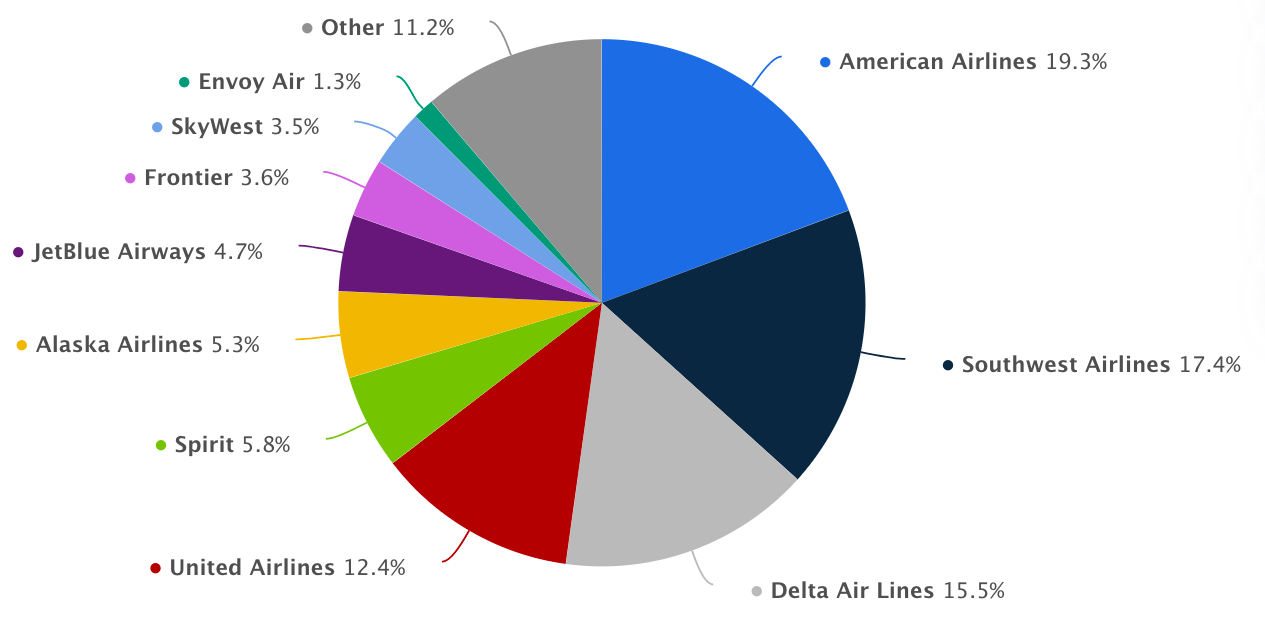
\includegraphics[width=9cm]{nayak_image1}
    \caption{American Airlines, Southwest Airlines, Delta Air Lines, and United Airlines may have an \textbf{oligopoly} on the market for air travel.}
    \label{fig:1}
    \end{minipage}
\end{figure}

	When studying most markets, economists assume that there exists \textbf{perfect competition}, where all products are the exact same, and buyers and sellers are so numerous that no single buyer or seller can influence the price. In these markets, firms are price takers, meaning that they must accept the market price, which is determined by supply and demand. On the other hand, oligopoly is an example of \textbf{market power}, which is a type of market failure that occurs when one or more firms can influence the price of a product. Since there is little competition, firms may be price makers, meaning they can artificially raise prices and consumers will still buy the product. Unlike with a monopoly, where the firm has no competition, firms in oligopolistic markets still have competitors, so their ability to raise prices is more limited. For example, if American Airlines were to raise their price drastically, travelers would simply switch to a different airline.

	Firms may use non-price competition to compete with other firms in an oligopolistic market, with methods like advertisement, branding, or location. In a perfectly competitive market, firms would likely not rely as much on non-price competition because every product would be the same. Granted, a perfectly competitive market is almost always an oversimplification, but there are markets where the products are extremely similar—for example, the market for salt. In a monopolistic market, the firm will not use methods of non-price competition because it has no competitors. Therefore, non-price competition is most common in oligopolistic markets, where the products are different, and there are a few firms competing with each other. To understand the firms’ decisions and interactions as they engage in this competition, we can call upon the science of strategy.


\noindent
\textbf{Game Theory}

\noindent
\emph{The Prisoners' Dilemma}

The most standard example of game theory is the prisoners’ dilemma, a situation in which two criminals are caught and taken into police custody. Here, we will call them Prisoner A and Prisoner B. In our example, the police have evidence that both individuals have committed a crime, say petty theft, that will put them in prison for 1 year. However, the police believe that both criminals have committed a worse crime, such as a major bank robbery. The prisoners are separated, so they cannot communicate, and they are given the following information:

\begin{itemize}
  \item If both confess to the bank robbery, both will serve 5 years in prison.
  \item If both refuse to confess, both will serve six months in prison for the lesser crime (petty theft).
  \item If one remains silent and the other confesses, the one who confesses will be set free, and the other will serve 10 years in prison.
\end{itemize}

We can see the dilemma in a matrix:

\begin{figure}[htp]
    \centering
    \begin{minipage}{9cm}
    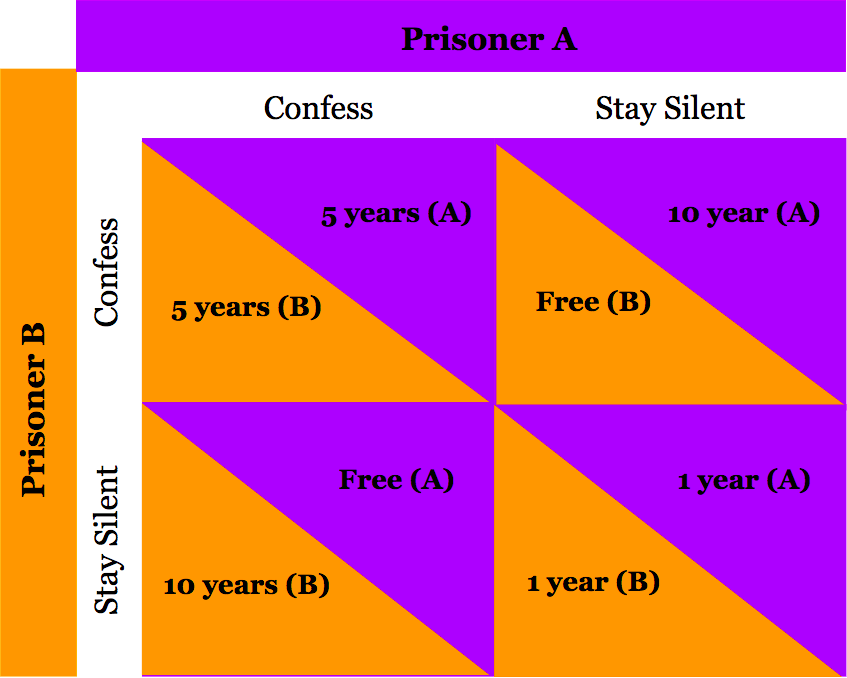
\includegraphics[width=9cm]{nayak_image2}
    \caption{The Prisoners’ Dilemma.}
    \label{fig:2}
    \end{minipage}
\end{figure}


    Since both prisoners are held separately and cannot communicate, they will act to maximize their own self-benefit. We can look at the situation from Prisoner A’s point of view. If Prisoner B confesses, Prisoner A’s best decision would be to confess and spend 5 years in jail instead of 10. If Prisoner B stays silent, Prisoner A should still confess so he can spend no time in jail instead of 1 year. Prisoner B will look at the situation in the exact same way. In this example of the prisoners’ dilemma, both prisoners have a \textbf{dominant strategy}, which is—in game theory—a strategy that is optimal no matter how other players act. Because both prisoners should confess regardless of the other prisoner’s decision, this is their dominant strategy. Acting in self-interest and unaware of the other individual’s decision, rational prisoners will confess even though they could have both remained silent to minimize their total prison time.

\noindent
\emph{Nash Equilibrium}

The case we have just examined demonstrates the \textbf{Nash Equilibrium}, where all players do not change their strategy, given the strategies of the other players. It is named after John Nash, an American mathematician whose thesis containing the equilibrium won him the Nobel Prize in Economic Sciences.

\begin{figure}[htp]
    \centering
    \begin{minipage}{9cm}
    
\includegraphics[width=9cm]{nayak_image3}
    \caption{John Nash in 2011 [2]}
    \label{fig:2}
    \end{minipage}
\end{figure}


In the years following the publication of Nash’s thesis in 1950, economists examining oligopoly have relied heavily on the ideas Nash outlined. We have seen how the equilibrium is present when studying prisoners’ decisions, and we can now extend these ideas to firms.

\noindent
\textbf{Oligopoly and Game Theory}

\noindent
\emph{Advertisement}

Let us consider a \textbf{duopoly}, an oligopoly where two firms control supply. These two firms—say Coke and Pepsi—dominate the market for soft drinks and engage in non-price competition in the form of advertisement. We can construct a \textbf{payoff matrix}, as we did with the prisoners’ dilemma, to examine possible outcomes in this hypothetical situation:

\begin{figure}[htp]
    \centering
    \begin{minipage}{9cm}
    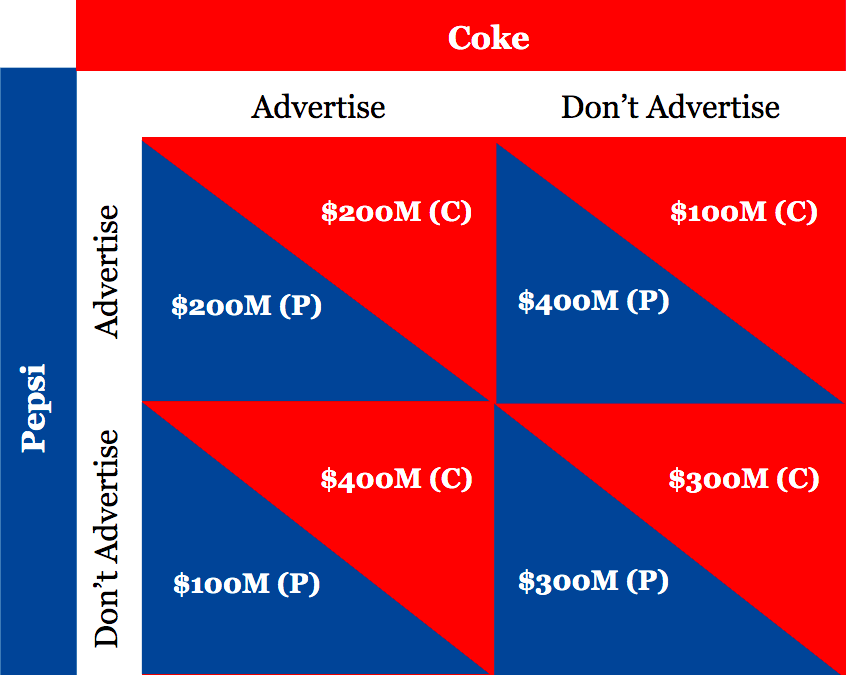
\includegraphics[width=9cm]{nayak_image4}
    \caption{A payoff matrix for Coke and Pepsi depending on their decision regarding advertisements.}
    \label{fig:2}
    \end{minipage}
\end{figure}

\pagebreak
As we can see in the matrix, the situation is very similar to the prisoners’ dilemma. If Pepsi does not advertise, Coke’s best strategy is to advertise, so they can gain \$400 million in profits instead of \$300 million. If Pepsi does advertise, Coke’s best strategy is to advertise, so they can gain \$200 million instead of \$100 million. Regardless of what Pepsi chooses to do, Coke should advertise: this is their dominant strategy. The situation from Pepsi’s point of view is exactly the same. This will lead to both firms advertising and gaining \$200 million in profits; this is a Nash equilibrium, since no firm will have an incentive to change their strategy, given what the other firm is doing.

Still, we can see that both Coke and Pepsi could have been better off if they had both chosen not to advertise (maybe they would have saved on the costs of creating and purchasing advertisements). We saw in the prisoners’ dilemma that the prisoners were isolated and could not speak to one another, so they could not devise a strategy together. But in this situation, could Coke and Pepsi discuss the situation with each other and increase both firms’ profits by not advertising? The answer is no: this would be \textbf{collusion}.

If firms in oligopoly were allowed to conspire with one another, forming what is called a \textbf{cartel}, they would simply band together and raise all of their prices collectively. For example, if Coke and Pepsi were the only two soft drinks, and both doubled their prices, consumers would have nowhere else to purchase soft drinks, so the firms would both increase their profits. However, this would be inefficient, since prices have been raised artificially, and it would also be unfair for consumers. To prevent situations like these from occurring, Congress has passed \textbf{antitrust laws}. Since they were first introduced in the United States in the late 1800s, these laws have encouraged competition and free markets. Still, they have not completely prevented firms from colluding, and even in the 21st century, there have been a handful of antitrust lawsuits.

\noindent
\textbf{Conclusion}

This article provided a brief overview of oligopoly and game theory. We investigated real-world examples of oligopolies and discussed market power. We introduced game theory and examined the classic example of the prisoners’ dilemma to illustrate the ideas of dominant strategy and a Nash equilibrium. Further, we constructed payoff matrices, discussed duopoly and market power, and we defined collusion, cartels, and antitrust laws.

The field of game theory and its applications in oligopoly are extensive. The science of strategy is a broad and far-reaching field, and as economists and game theorists continue to analyze behavior and markets, the applications will only continue to expand.



\pagebreak
\begin{thebibliography}{3}

\bibitem{} 
https://www.statista.com/statistics/250577/domestic-market-share-of-leading-us-airlines/

\bibitem{}
https://commons.wikimedia.org/wiki/File:John\_Forbes\_Nash,\_Jr..jpg

\bibitem{}
Mankiw, N. Gregory. Principles of Microeconomics. 8th ed., CENGAGE Learning Custom Publishing, 2016.

\end{thebibliography}
